\documentclass[10pt,a4paper]{article}

% === PAQUETES === (((
\usepackage{amsmath}
\usepackage[shortlabels]{enumitem}
\usepackage{amsfonts}
\usepackage{ragged2e}
\usepackage{subfigure}
\usepackage{amssymb}
\usepackage{slashbox}
\usepackage{multirow}
\usepackage{multicol}
\usepackage{fontspec}
\usepackage{fullpage}
\usepackage{graphicx}
\usepackage{titlesec} 
% \usepackage{setspace}
\usepackage{dsfont}
% \usepackage{bookmark}
% )))

% === TIPOGRAFÍA === (((
\setmainfont[
  BoldFont       = bodonibi,
	ItalicFont     = Century modern italic2.ttf,
	BoldItalicFont = bodonibi,
	SmallCapsFont  = lmromancaps10-regular.otf
]{Century_modern.ttf}
% )))

% === COMANDOS === (((
\newcommand{\dis}{\displaystyle}
\newcommand{\qed}{\hspace{0.5cm}\rule{0.16cm}{0.4cm}}
\newcommand{\micita}[1]{\([\)\cite{#1}\(]\)}
\newcommand{\operator}[1]{\mathop{\vphantom{\sum}\mathchoice{ \vcenter{\hbox{\huge $#1$}} }
{\vcenter{ \hbox{\Large $#1$}} }{#1}{#1}}\displaylimits}
\newcommand{\suma}{\operator{ 
\includegraphics[scale=0.09]{IMAGENES/Sigma.png}} }
\DeclareSymbolFont{italics}{\encodingdefault}{\rmdefault}{m}{it}
\DeclareSymbolFontAlphabet{\mathit}{italics}
\ExplSyntaxOn
\int_step_inline:nnnn { `A } { 1 } { `Z }
 {  \exp_args:Nf \DeclareMathSymbol{\char_generate:nn{#1}{11}}{\mathalpha}{italics}{#1} }
\int_step_inline:nnnn { `a } { 1 } { `z } {  \exp_args:Nf \DeclareMathSymbol{\char_generate:nn{#1}{11}}{\mathalpha}{italics}{#1}}
\ExplSyntaxOff
% )))

% === SECCIONES === (((
\titleformat*{\section}{\large\normalfont\bfseries}
\titleformat*{\subsection}{\large\itshape \centering}
% \setcounter{secnumdepth}{0}
\renewcommand*{\contentsname}{\large\textbf{CONTENIDOS.}}
\usepackage[nottoc,numbib]{tocbibind}
\renewcommand{\refname}{REFERENCIAS.}
\renewcommand{\tablename}{Tabla}
\renewcommand{\figurename}{Figura}
% )))

% === PORTADA === (((
% \pagestyle{empty}
\newcommand{\portada}{
\addfontfeature{LetterSpace=-5}
  \begin{titlepage}
  \centering
  \begin{figure}
    \centering
    
\includegraphics[scale=0.5]{IMAGENES/logo_uaa.png}  
  \end{figure}
  {\bfseries\Large\MakeUppercase{\textit{Universidad Autónoma de Aguascalientes.}} \par}
  \vspace{1cm}
  {\Large Centro de Ciencias Básicas. \vspace{0.5cm}\\[2mm]
  Departamento de Matemáticas y Física.\vspace{0.5cm}\\[2mm]
  Licenciatura en Matemáticas Aplicadas.\vspace{0.5cm}\\[2mm]
  Práctica 6.\par}
  \vspace{1.5cm}
  {\bfseries\Huge Experimento de Young. \par} % title
  \vspace{1.5cm}
  {\itshape\Large Óptica. \\Prof. Mariana Alfaro Gómez.\par}
  % {\itshape\Large Variable Compleja I. \\Prof. Fausto Arturo Contreras Rosales.\par}
  % {\itshape\Large Métodos Numéricos II. \\Prof. Manuel Ramírez Aranda.\par}
  % {\itshape\Large Diseño de Experimentos. \\Prof. Angélica Hernández Quintero.\par}
  % {\itshape\Large Filosofía de la Investigación Científica. \\Prof. Jesús Mariano Rodríguez Muñoz.\par}
  \vfill
  % {\Large \textit{Por Erick I. Rodríguez Juárez.}\par}
		\begin{flushleft}
		\Large
		Alumnos:\\
		\textit{Carlos Francisco Guzmán Barba.}\\
		\textit{Erick Ignacio Rodríguez Juárez.}\\
		\textit{Manuel Alejandro Siller Landin.}
		\end{flushleft}
	% {}  % {\Large \textit{Por Erick I. Rodríguez Juárez.}\par}
  \vfill
		\begin{flushright}
		{\Large Realización: 2\(/\)05\(/\)22. \par} % date
		{\Large Entrega: 16\(/\)05\(/\)22. \par} % date
		\end{flushright}
  \end{titlepage} 
	% \thispagestyle{empty}
	% \doublespacing
	% \tableofcontents
	% \singlespacing
	% \newpage
} 
% )))

\begin{document}

\portada

\section{RESUMEN.} % (((
Para esta práctica se construyó, mediante un arreglo experimental, un generador de ondas usando un hilo el cual nos permitió visualizar ondas estacionarias de las que podíamos variar tanto su frecuencia como su tensión, puesto que estuvo sujeto en uno de sus extremos mediante un porta pesas del cual se le pudo variar la masa, para obtener sus armónicos. Con lo cual, vimos que al tener una variación de $0.5\;Nw$ en la tensión de la cuerda, se produjo un cambio de entre \([(528 \pm 16.385), (562\pm 61.007)]\;cm/s\) en el valor de la velocidad para la onda producida por la cuerda, obteniendo así que entre más tensión se tenga sobre la cuerda, mayor será la velocidad de la onda que esta genere.
% )))

\section{INTRODUCCIÓN.} % (((

\subsection{--- Propiedades de la Oscilación de una Cuerda ---} % (((
\label{sub:cuerda}
\begin{figure}[ht]
	\begin{minipage}{0.45\linewidth}
		\addfontfeature{LetterSpace=-5}
		Considérese el movimiento vertical de una cuerda sujeta a una tensión uniforme \(T\) en toda su longitud.
		Hagamos los Diagramas de Cuerpo Libre (DCL) en los puntos \(k\) y \(x\) del eje horizontal, tal como lo indica la Figura \ref{fig:cuerdita} (original en \micita{alonso_finn_1}).
		Si \(\varphi : \mathds{R} \times \mathds{R} \longrightarrow \mathds{R}\), es la función, de onda, entonces el vector \(T\) es paralelo a su derivada, 
		\[
			\begin{array}{rcl}
				\dfrac{\partial \varphi}{\partial x} (x) = \dfrac{T_y}{T_x} \approx \dfrac{T_y}{T} \\[6mm]
				\dfrac{\partial \varphi}{\partial x} (k) = \dfrac{T\,'_y}{T\,'_x} \approx \dfrac{T\,'_y}{T}
			\end{array}
		\]
	\end{minipage}
	\begin{minipage}{0.55\linewidth}
		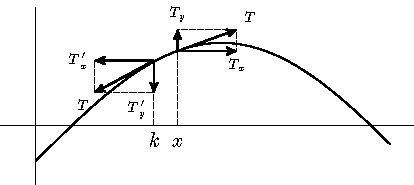
\includegraphics[width= \linewidth]{1_INTRO/2/tikz.pdf}
		\caption{Fuerzas alrededor del punto \(k\) en la cuerda.}
		\label{fig:cuerdita}
	\end{minipage}
\end{figure}%\\
Entonces, en el segmento de cuerda \([k,x]\) se experimentará la siguiente cantidad de fuerza vertical,
\[
	F_y = T_y-T\,' _y = T \cdot \bigg[\dfrac{\partial \varphi}{\partial x} (x) - \dfrac{\partial \varphi}{\partial x} (k)\bigg]
\]
Notamos además, que si la cuerda tiene una densidad de masa \(\mu\) por unidad de longitud, por tanto \(m= \mu (x-k)\), en el segmento \([k,x]\).
En virtud de la Primer Ley de Newton tenemos:
\[
	F_y = ma = \big[\mu (x-k)\big] \cdot y'' = \mu (x-k) \cdot \dfrac{\partial ^2 \varphi}{\partial t^2}.
\]
Dado que las dos ecuaciones anteriores son válidas para todo \(x\), luego, también lo son cuando \(x \longrightarrow k\).
\begin{align*}
	\mu (x-k) \cdot \dfrac{\partial ^2 \varphi}{\partial t^2} &= T \cdot \bigg[\dfrac{\partial \varphi}{\partial x} (x) - \dfrac{\partial \varphi}{\partial x} (k)\bigg] \\[6mm]
	\therefore \hspace{1cm} \dfrac{\partial ^2 \varphi}{\partial t^2} &= \dfrac{T}{\mu} \cdot \dis\lim_{x\rightarrow k} \dfrac{\frac{\partial \varphi}{\partial x} (x) - \frac{\partial \varphi}{\partial x} (k)}{x-k} = \dfrac{T}{\mu} \cdot \dfrac{\partial ^2 \varphi}{dx^2}.
\end{align*}
Así, \(\varphi\) satisface la ecuación de onda
\begin{equation}
	\dfrac{\partial^2 f}{\partial t^2} = v^2 \dfrac{\partial ^2f}{\partial x^2}
	\label{eq:onda}
\end{equation}
con
\begin{equation}
	v = \sqrt{T/ \mu}
	\label{eq:velocidad}
\end{equation}
% )))

\newpage

\subsection{--- Cuerda con un Extremo Fijo ---} % (((
\label{sub:cuerd_var}
\begin{figure}[ht]
	\begin{minipage}{0.4\linewidth}
		\addfontfeature{LetterSpace=-5}
		Supóngase que se tiene una cuerda en \([0, \infty)\) con un extremo fijo en el origen \(P\), que propaga una onda unidimensional transversal en un mismo medio.
		Tal como en la Figura \ref{fig:extr_libre}. \\[2mm]
		Sea la función de onda inicial \(\varphi_1 :[0, \infty ) \times \mathds{R} ^+ \longrightarrow \mathds{R}\), y la función que es el reflejo de tal onda, \(\varphi _2: [0, \infty ) \times \mathds{R} ^+ \longrightarrow \mathds{R}\).
		Entonces
		\[
			\begin{array}{rcl}
				\varphi _1(x,t) & = & A \sin (kx+ \omega t) \\
				\varphi _2(x,t) & = & A \sin (kx- \omega t) .
			\end{array}
		\]
		puesto que \(\varphi _1\), y \(\varphi _2\) tienen la misma amplitud, y se desplazan a la misma rapidez.
		Sin embargo, dado que una es la reflexión de la otra, entonces son simétricas en el tiempo.
		Note que,
		\[
			\dfrac{\partial ^2 \varphi _1}{\partial x^2} = -k^2 \cdot \varphi _1 \hspace{5mm} \;\land\; \hspace{5mm} \dfrac{\partial ^2 \varphi _1}{\partial t^2} = -\omega ^2 \cdot \varphi _1
		\]
	\end{minipage}\hspace{5mm}
	\begin{minipage}{0.6\linewidth}
		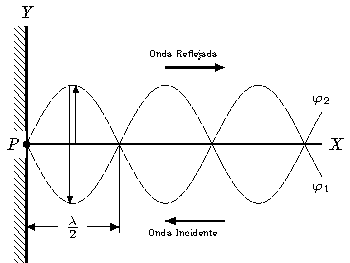
\includegraphics[width= \linewidth]{1_INTRO/3/tikz.pdf}
		\caption{Reflexión de una onda transversal en el punto \(P\).}
		\label{fig:extr_libre}
	\end{minipage}
\end{figure}
Así, \(\dfrac{1}{k^2} \dfrac{\partial ^2 \varphi _1}{\partial x^2} = \dfrac{1}{\omega ^2} \dfrac{\partial ^2 \varphi _1}{\partial t^2} \implies \dfrac{\partial ^2 \varphi _1}{\partial t^2} = \dfrac{\omega ^2}{k^2} \cdot \dfrac{\partial ^2 \varphi _1}{\partial x^2}\).
Es decir, \(\varphi _1\) satisface (\ref{eq:onda}), con \(v= \omega /k\).
Dadas las definiciones de \(\lambda = 2 \pi /k\) como la \textit{longitud de periodicidad de la onda}, y \(f = \omega /2 \pi\) como el recíproco de la \textit{periodicidad temporal}, se tiene
\begin{equation}
	v = \lambda \cdot f
	\label{eq:velocidad_1}
\end{equation}
% )))

\subsection{--- Ondas Estacionarias Unidimensionales ---} % (((
\label{sub:ondas_estacionarias}
\begin{figure}[ht]
\begin{minipage}{0.5\linewidth}
	\centering
	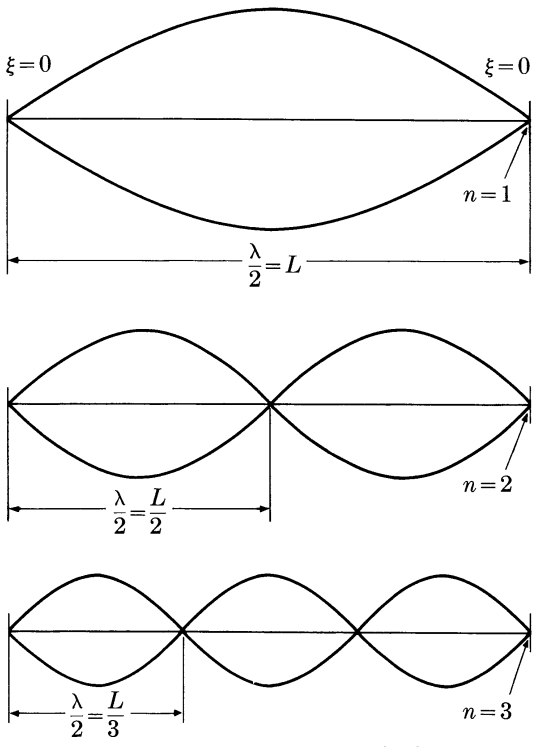
\includegraphics[width= 0.8 \linewidth]{1_INTRO/estacionaria.png}
	\caption{Ondas estacionarias en una long. \(L\) fija.}
	\label{fig:estacionaria}
\end{minipage}
\begin{minipage}{0.5\linewidth}
	\addfontfeature{LetterSpace=-5}
	Para las funciones de la Figura \ref{fig:extr_libre}, la onda total es (por el principio de superposición) la suma algebraica siguiente
	\[
		\varphi (x,t) = \varphi _1(x,t) + \varphi _2(x,t) = 2A \sin kx \cdot \cos \omega t.
	\]
	(dado que \(\sin \alpha + \sin \beta = 2 \sin (\alpha + \beta) /2 \cdot \cos (\alpha - \beta) /2\)).
	Observamos que la función \(\varphi\), no depende de \(kx \pm \omega t\), sin embargo, es una onda, puesto que satisface (\ref{eq:onda}) (dado que (\ref{eq:onda}) es una ecuación diferencial lineal).
	Por este motivo, a \(\varphi\) se le llama \textbf{función de onda estacionaria}. \\[2mm]
	Consideremos el caso en donde ambos extremos están fijos en el eje horizontal a una distancia \(L\).
	Cuando \(\cos \omega t = 1\), se tiene la amplitud máxima en un punto fijo \(x\), \textit{i.e.} \vspace{-2mm}
	\[
		\varphi _{max} (x) = 2A \sin kx.
	\]
	Notamos que se tendrá \(\varphi _{max} = 0\), cuando \(kx = n \pi\), con \(n \in \mathds{Z}\).
	Los puntos \(x = n \pi /k = n \lambda /2\), se llaman \textbf{nodos}.
	En la Figura \ref{fig:estacionaria}, se forma una sucesión de ondas \(\varphi _n\), cada una, con nodos en \(x =0, L/ n,2L/n,3L/n, \;\ldots,\; L\).
	\begin{equation}
		\lambda _n/2 = L/n \;\implies\; \lambda _n = 2L/n.
		\label{eq:nodos}
	\end{equation}
\end{minipage}
\end{figure}
\newpage
Y si en la sucesión construida en la Figura \ref{fig:estacionaria}, la onda siempre viaja a la misma velocidad \(v\), se tendrá por las ecuaciones (\ref{eq:velocidad_1}) y (\ref{eq:nodos}), \(f_n = \dfrac{v}{\lambda _n} = \dfrac{v}{(2L/n)} = n\dfrac{v}{2L}\).
Como \(f_1=v/(2L)\), entonces
\begin{equation}
	f_n = n f_1.
	\label{eq:frecuencia}
\end{equation}
Consecuentemente, por la ecuación (\ref{eq:velocidad}) para la función de onda \(\varphi _n\), \(f_n = n \dfrac{v}{2L} = n \dfrac{\sqrt{T/ \mu}}{2L}\), e implica que
\begin{equation}
	T = \bigg(\dfrac{f_n \cdot 2L}{n}\bigg) ^2 \cdot \mu = \dfrac{4 \mu f\,_n^2L^2}{n^2}.
	\label{eq:tension}
\end{equation}
La sucesión de funciones \(\varphi _n\), se les llaman \textit{armónicos}, y a \(\varphi _1\), se le llama \textit{armónico fundamental}.
% )))

\subsection{--- Método de Mínimos Cuadrados ---} % (((
Sean \((x_i, y_i)\), con \(i=1, \;\ldots,\; n\), un conjunto de \(n\) puntos distintos.
Se desea encontrar la recta \(f(x) =ax+b\), que minimice la suma de los cuadrados del error \(E(a,b) = \dis\suma_{i=1} ^n \big(ax_i+b -y_i\big) ^2\).
Para ello, se obtiene el sistema lineal de las ecuaciones diferenciales \(\dfrac{\partial E}{\partial a} =0\), y \(\dfrac{\partial E}{\partial b} =0\).
Cuyas soluciones son las siguientes.
\[
	\begin{array}{rcl}
		a&=&\dfrac{n\left(\dis\suma_{i=1}^n x_i y_i\right)-\left(\dis\suma_{i=1}^n x_i \right)\left(\dis\suma_{i=1}^n y_i\right) }{n \left(\dis\suma_{i=1}^n x_i^2\right)-\left(\dis\suma_{i=1}^n x_i\right)^2} \\[1.6cm]
		b&=&\dfrac{\left(\dis\suma_{i=1}^n x_i^2\right)\left(\dis\suma_{i=1}^n y_i\right)-\left(\dis\suma_{i=1}^n x_i \right)\left(\dis\suma_{i=1}^n x_i y_i\right) }{n \left(\dis\suma_{i=1}^n x_i^2\right)-\left(\dis\suma_{i=1}^n x_i\right)^2}
	\end{array}
\]
Consúltese \micita{mont}, para la resolución del sistema lineal.
% )))

\subsection{--- Métodos de Análisis Experimental ---} % (((
\label{sub:analisis_exp}
El objetivo del sistema físico a plantear es obtener de forma experimental el efecto que provoca la tensión de una cuerda, a la velocidad de propagación de la función de onda.
Se pudo controlar siempre la magnitud y dirección de la tensión debido a que se estableció un juego de una polea (conectada a la cuerda de análisis), que, sin intervención de ninguna otra fuerza (más que la gravitacional), permitió variar el peso total ejercido a través del sistema.
Por lo tanto, se espera tener estimaciones cercanas de la tensión \(T\), a través de la medición directa de los elementos en las ecuaciones (\ref{eq:velocidad}) y (\ref{eq:tension}).
Para trabajarse con \(Nw=kg \cdot m/s^2\), las unidades (de conversión) usadas para el reporte de los datos relacionados a la tensión estarán en \(kg\) (para la masa) y en \(m\) (para las longitudes).
% )))

% )))

\section{METODOLOGÍA.} % (((
\label{sec:metodologia}
\begin{itemize}
	\item La incertidumbre del flexómetro es de $ \dfrac{0.1cm}{2}=0.05cm $.
	\item La incertidumbre de la báscula es de $ \dfrac{0.1 g}{2}=0.05 g $.
	\item La incertidumbre del generador de ondas es de $ \dfrac{0.1 Hz}{2}=0.05 Hz $.
\end{itemize}
Las Figuras \ref{fig:met1} y \ref{fig:met2} muestran la configuración para el dispositivo experimental usado.
Se posiciona mediante dos soportes universales el generador de ondas y la polea de tal manera que, partiendo de un extremo de un hilo al amarrarlo desde la parte movible del generador de ondas, hasta entrar en contacto con la polea para que quede horizontal con respecto a la mesa de trabajo, se pueda terminar amarrando un porta pesas en el otro extremo del hilo.
\begin{figure}[hbt!]
	\centering
	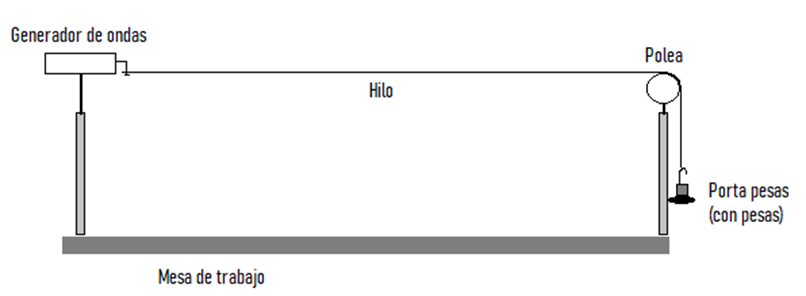
\includegraphics[width= 0.8 \linewidth]{2_METODO/1}
	\caption{Configuración inicial del experimento.}
	\label{fig:met1}
\end{figure}
\begin{figure}[hbt!]
	\centering
	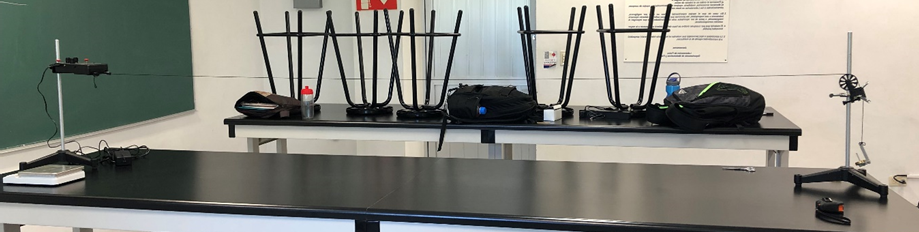
\includegraphics[width= 0.8 \linewidth]{2_METODO/2}
	\caption{Foto de la configuración inicial del dispositivo experimental.}
	\label{fig:met2}
\end{figure}\\
\begin{figure}[hbt!]
\begin{minipage}{0.4\linewidth}
	\addfontfeature{LetterSpace=-5}
	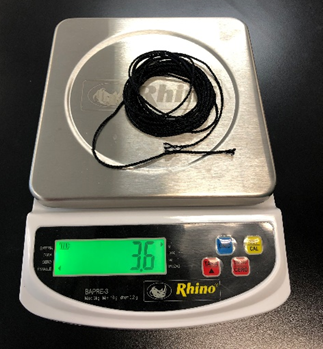
\includegraphics[width= 0.9 \linewidth]{2_METODO/3}
	\caption{Se empleó una báscula para poder obtener la masa del hilo total usado en experimento.}
	\label{fig:met3}
\end{minipage}
\begin{minipage}{0.6\linewidth}
	\addfontfeature{LetterSpace=-5}
	Para poder justificar las operaciones del marco teórico fue necesario obtener la masa y su longitud primeramente de un pedazo de hilo lo suficientemente largo para elaborar la configuración para el dispositivo experimental.
	La forma de obtener la masa del hilo se muestra en la Figura \ref{fig:met3}. \\[2mm]
	En seguida, al ya tener listo el dispositivo experimental, se midió la longitud del hilo desde la parte movible del generador de ondas, hasta la región de contacto del hilo con la polea. \\[2mm]
	Como siguiente paso se realizaron varias mediciones variando la combinación del porta pesas con las pesas y las frecuencias para obtener las longitudes de onda respectivas a los armónicos del hilo.
\end{minipage}
\end{figure}\\
Primeramente, con una combinación de pesas de \(M=150gr\), con una \(f=29Hz\) y en seguida para una de \(M=200gr\) y \(f=33.7Hz\) para finalmente proceder a obtener los valores de las frecuencias para diferentes armónicos (9 armónicos distintos) variando 5 veces la tensión en el hilo causado por la masa de las pesas.
% )))

\newpage

\section{RESULTADOS.} % (((
 Se tuvieron las siguientes observaciones como parte del armado del sistema experimental:
 \begin{itemize}[noitemsep]
	\item La longitud total de la cuerda era de $ (331.5\pm 0.05) cm $.
	\item La longitud de \(L\) en el experimento (continuando con la notación de la sección \ref{sub:ondas_estacionarias}), fue de $ L = (267 \pm 0.05) cm $.
	\item La masa de la cuerda era de $( 3.6 \pm 0.05)g $.
	\item La densidad de masa de la cuerda resultó entonces de (véase apéndice \ref{sub:densidad}).
	$$\mu=\left(0.0108\pm0.0001\right)\dfrac{g}{cm}=(0.00108\pm 0.00001)\dfrac{kg}{m}$$
 \end{itemize}
Luego, para obtener la medición de la longitud de la onda estacionaria producida por el generador, con dos valores de masa distintos pero con el mismo armónico ($n=4$), se obtuvieron los siguientes resultados (Tabla \ref{tab:primera}).
\begin{table}[ht]
\centering
\caption{Resultados obtenidos de las mediciones.}
	\begin{tabular}{|l|c|c|}
			\hline
			Dato Experimental & Experimento 1 & Experimento 2 \\ 			\hline
			Masa del portapesas & $ 0.005 kg $ & $ 0.005 kg $ \\ 			\hline
			Masa agregada $ m $& $ 0.150 kg $ & $ 0.200 kg $  \\ 			\hline
			Masa total $ M $ & $ 0.155kg $ & $ 0.205kg $  \\ 			\hline
			Tensión en la cuerda $ T $ & $ 1.52055 Nw $  & $ 2.0110 Nw$ \\ 			\hline
			Valor de la frecuencia $ f $ & $ (29\pm 0.05)Hz$  & $ (33.7\pm 0.05)Hz $ \\ 			\hline
			Longitud de onda $ \lambda $ & $ (134\pm0.05)cm $ & $ (131\pm0.05)cm $  \\ 			\hline
	\end{tabular}
	\label{tab:primera}
\end{table}\\
Para los cálculos de la velocidad con las fórmulas (\ref{eq:velocidad_1}) y (\ref{eq:velocidad}) de la práctica, los resultados se colocan en la Tabla \ref{tab:segunda}.\vspace{-5mm}
\begin{table}[ht]
	\small 
\centering
\caption{Cálculo de la velocidad de onda.}
	\begin{tabular}{|c|c|c|c|c|c|c|c|}
		\hline
		Experi-& $ \lambda $ $ (cm)$ & $ f $ $ (Hz)$ & $ v_a=\lambda\cdot f $ & $ T $ & $ \mu  (\frac{kg}{m})$ & $ v_b=\sqrt{\frac{T}{\mu}} $ & Diferencia \\
		mento & $ \pm 0.05cm $ & $ \pm 0.05 Hz $ & $ (\frac{cm}{s}) $ & $ (Nw) $ & $ \pm 0.00001\frac{kg}{m} $ & $ (\frac{cm}{s}) $ & $ |v_a-v_b| (\frac{cm}{s}) $ \\ 		\hline
		1 & 134 & 29 & $ 3886\pm8.15 $ & 1.52055 & $0.00108$ & $ 3741.889\pm 26.26753 $ & $ 144.111 $ \\ 		\hline
		2 & 131 & 33.7 & $ 4414.7\pm8.235 $ & 2.0110 & $0.00108$ & $ 4303.303\pm 34.74093 $ & $ 111.397 $ \\ 		\hline
	\end{tabular}
	\label{tab:segunda}
\end{table}\\
Luego, para una masa fija de $ 155g $, se obtuvo que la frecuencia del armónico fundamental ($ n=1 $) era de $$f_1=(7\pm0.05)Hz$$
Empleando la fórmula (\ref{eq:frecuencia}) se obtiene el valor esperado de \(f_n\), y se obtiene el error absoluto y relativo con respecto al valor esperado. Los resultados se reportan en la Tabla \ref{tab:tercera}.\vspace{-5mm}
\begin{table}[hbt!]
	\centering
	\caption{Frecuencia en los modos de oscilación.}
	\begin{tabular}{|l|l|l|l|l|}
		\hline
		Armónico & $ f $ esperada & $ f $ observada en $Hz$  & Error &Error  \\
		$ n $ & en $ Hz $ & $\pm 0.05 Hz $ & absoluto (\(Hz\)) & relativo\\  		\hline
		2 & $ 14 \pm 0.1$ & 15 & $ 1\pm 0.15 $ & $7.1428$ \textsc{\%}\\ 		\hline
		3 & $ 21 \pm 0.15$ & 22 & $ 1\pm 0.2 $ & $4.7619$ \textsc{\%}\\  		\hline
		4 & $ 28 \pm 0.2$ & 29 & $ 1\pm 0.25$ & $3.5714$ \textsc{\%}\\ 		\hline
	\end{tabular}
	\label{tab:tercera}
\end{table}\\
Para la siguiente parte del experimento, se optó por dejar una frecuencia fija de $f=(22\pm 0.05) Hz$, y haciendo variar la masa del portapesas para obtener distintos armónicos, los resultados para la tensión son de la Tabla \ref{tab:cuarta}.
Observar que no se realizó la medición experimental de las masas \(m\),
\begin{table}[hbt!]
	\centering
	\caption{Tensión en la cuerda para distintas masas con misma frecuencia.}
	\begin{tabular}{|*{3}{l|}}
		\hline
		Armónico \(n\) & Masa \(m\) (\(kg\)) & Tensión \(T\) (\(Nw\)) \\ \hline
		3& 0.155 & 1.52055 \\ 		\hline
		4& 0.105 & 1.03005 \\ 		\hline
		5& 0.055 & 0.53955 \\ 		\hline
		6& 0.025 & 0.24525 \\ 		\hline
	\end{tabular}
	\label{tab:cuarta}
\end{table}
\newpage
Luego, se realizaron las gráficas de $ T $ vs. $ n $ y $ T $ vs. $ 1/n^2 $, donde $ n $ representa el número de armónico.
Tales gráficas se muestran en las Figuras \ref{fig:graf1}, y \ref{fig:graf2}.
\begin{figure}[hbt!]
	\centering
	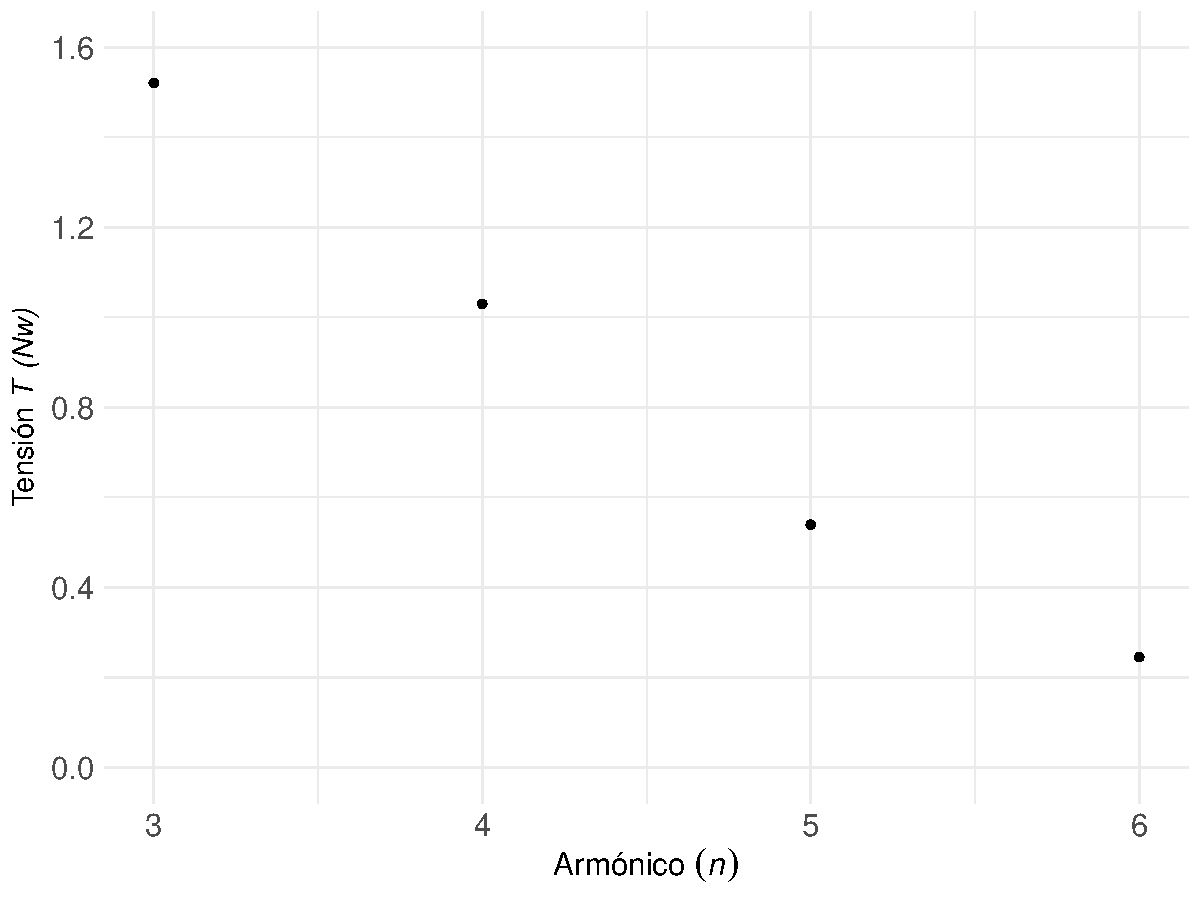
\includegraphics[width= 0.7\linewidth]{3_RESULTADOS/T vs n.pdf}
	\caption{$T$ vs. \(n\).}
	\label{fig:graf1}
\end{figure}\\
\begin{figure}[hbt!]
	\centering
	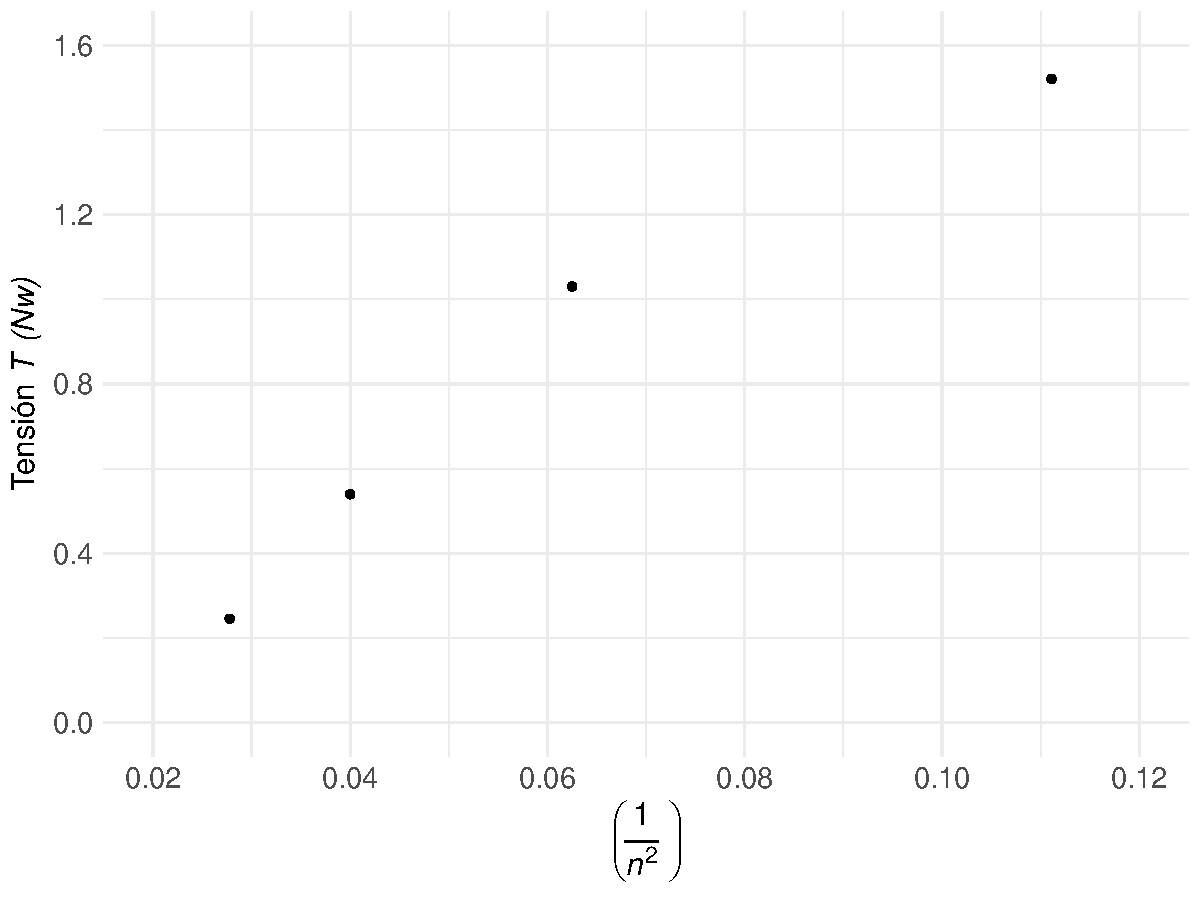
\includegraphics[width= 0.7\linewidth]{3_RESULTADOS/T vs n2.pdf}
	\caption{$T$ vs. $ \left(\dfrac{1}{n^2}\right) $.}
	\label{fig:graf2}
\end{figure}
\newpage
A partir de esta última relación, se obtuvo la estimación de la recta por mínimos cuadrados que se aproximara a estas observaciones, resultando que
$$ T=[(14.90009\pm 2.29002) Nw]\left(\dfrac{1}{n^2}\right)-(0.06533\pm 0.15625) Nw $$ 
La gráfica entonces queda en la Figura \ref{fig:graf3}.
\begin{figure}[ht]
	\centering
	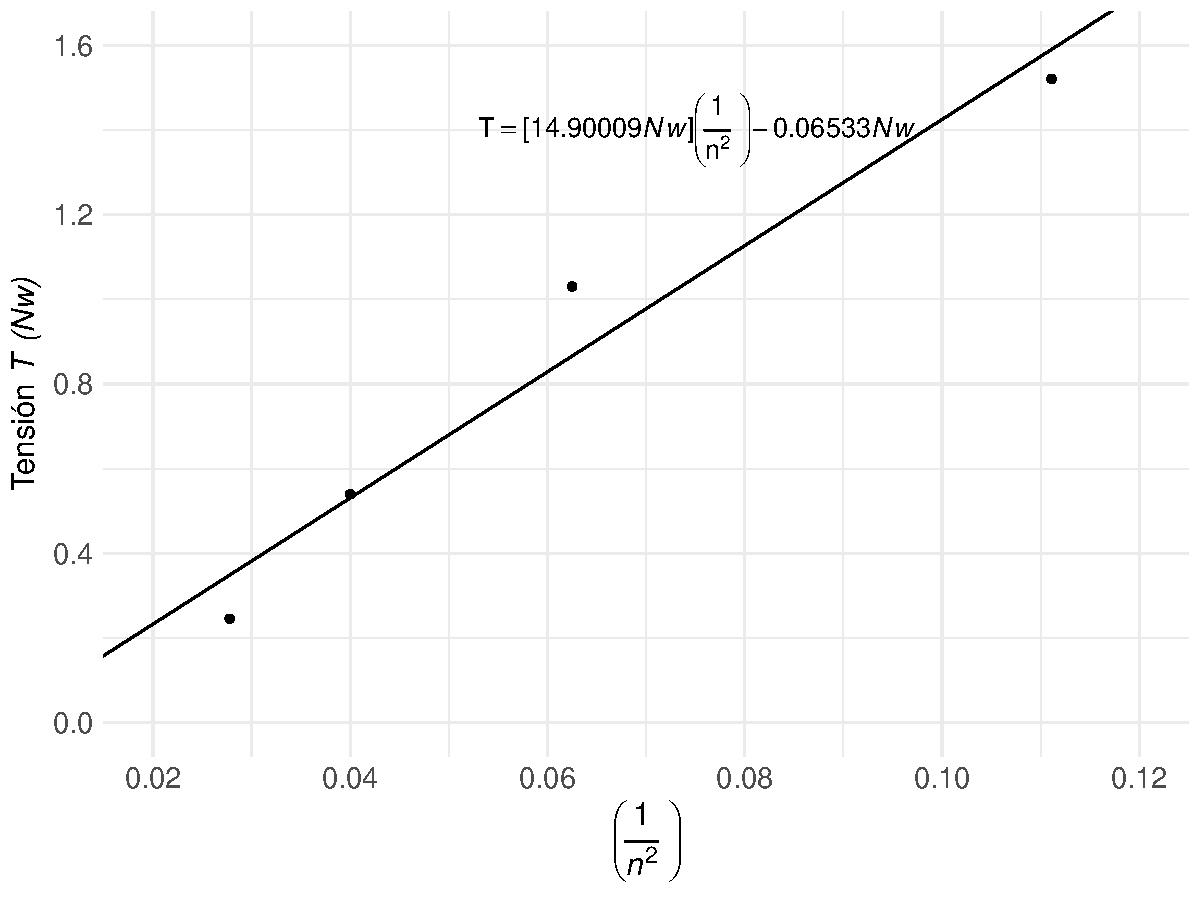
\includegraphics[width= 1\linewidth]{3_RESULTADOS/T vs n2 2.pdf}
	\caption{Estimación por mínimos cuadrados.}
	\label{fig:graf3}
\end{figure}\\
Luego, a partir del valor de la estimación de la pendiente, así como de la fórmula (\ref{eq:tension})
$$T=\left(4\mu f\,^2 L^2\right)\left(\dfrac{1}{n^2}\right)$$
se puede hacer una estimación para la densidad de masa lineal de la cuerda empleada.
Haciendo la estimación de $ \mu $ a partir de esto (véase el apéndice \ref{sub:nueva_estim} para los cálculos), se obtuvo que 
$$\mu=(0.00107\pm0.0001)\dfrac{kg}{m}$$
Comparando este valor con el obtenido al inicio de los resultados, se tiene tan solo una diferencia de 
$$|0.00108-0.00107|\dfrac{kg}{m}=0.00001\dfrac{kg}{m}$$
% )))

\newpage

\section{DISCUSIÓN DE RESULTADOS Y CONCLUSIONES.} % (((
Durante el desarrollo de este experimento, en el cual se sujetó el extremo de una cuerda a un generador de ondas y el otro extremo a un portapesas a través de una polea, fue posible observar de manera clara la generación de ondas estacionarias con distintos modos de oscilación (denominados “armónicos”) conforme la frecuencia era modificada.
Al formarse las oscilaciones en la cuerda, se logró obtener dos mediciones distintas de la longitud de onda correspondientes a frecuencias y masas distintas (ver tabla 1).
Además, al conocerse la masa del portapesas, se pudo determinar la tensión existente sobre la cuerda, y dado que la densidad de masa lineal de la cuerda también fue posible estimarla con los datos del experimento, se obtuvieron entonces dos posibles estimaciones para la velocidad de la onda (ver tabla 2).  \\[2mm]

Aunque teóricamente ambas ecuaciones son viables para el cálculo de la velocidad, la diferencia entre ambas fue mayor a $1 \frac{m}{s}$  para los dos experimentos realizados, por lo que podría haberse obtenido entonces una medición incorrecta de los datos experimentales, y la cual se atribuye principalmente debido a la frecuencia y/o la longitud de onda.
Por ejemplo, si se observa la tabla 3 (correspondiente a los valores de la frecuencia), se observa que no están coincidiendo los valores medidos con los esperados de manera teórica, a pesar de que los errores relativos sean menores al $10$\textsc{\%}. \\[2mm]

Además, las oscilaciones de la cuerda presentaron interferencia, y ésta provocaba que las ondas tuvieran un movimiento de precesión, y así, se obtuvo un movimiento tridimensional en el experimento.
Sin embargo, las ondas transversales pueden considerarse mediante una proyección unidimensional.
Tales perturbaciones también provocaron imprecisiones sobre la ubicación de los nodos a lo largo de la longitud $L$.
Lo recomendado es fijar los soportes universales a la mesa mediante prensas para minimizar las vibraciones y, además, intentar tomar capturas mediante fotos de las ondas de tal forma que a escala sea más fácil obtener dichas mediciones. \\[2mm]

En cambio, para el cálculo de dicha velocidad con la fórmula (2), no se obtuvieron las incertidumbres de las masas de las pesas,  por lo que el valor de la tensión en la cuerda se consideró preciso.
En adición, al realizar las gráficas de esta tensión contra los modos de oscilación (Figuras 4 y 5)  se puede observar una relación lineal que, a su vez, permitió obtener una segunda estimación completamente distinta de la densidad de masa de la cuerda y que era prácticamente igual a la calculada al inicio de los resultados, puesto que sólo difieren por $0.00001 \;kg/m$. Sin embargo, las incertidumbres finales $v_b$ fueron mayores debido al cálculo de la incertidumbre de la función $f(x)=\sqrt{x}$.
Y dado que la ecuación (3), $v_a=\lambda f$, requiere menos operaciones para el cálculo de las incertidumbres finales, terminó siendo más precisa (véase la Tabla 2, y el apéndice 7.4). \\[2mm]

Sin embargo, vemos que al final (nuevamente en la tabla 2) una variación de $0.5\;Nw$ en la tensión de la cuerda, produce un cambio de entre \([(528 \pm 16.385), (562\pm 61.007)]\;cm/s\) en el valor de la velocidad para la onda producida por la cuerda obtenidos de la ecuación (3) y (2) respectivamente, y que también va de la mano con los valores de la frecuencia y la longitud de la onda.
Así pues, con este experimento se concluye que entre más tensión se tenga sobre la cuerda mayor, será la velocidad de la onda que esta genere, tal como se esperaba en la ecuación (2).
% )))

% === REFERENCIAS === (((
\bibliography{Referencias}
\bibliographystyle{unsrt}
% )))

\section{APÉNDICE.} % (((
	\subsection{--- Propagación de la Incertidumbre ---}
	
	La propagación de la incertidumbre para la suma, el producto y un cociente están dadas (respectivamente) por
	\begin{align*}
		(x\pm \delta x)\pm(y\pm \delta y)&=(x\pm y)\pm(\delta x+\delta y)\\\\
		(x\pm\delta x)(y\pm\delta y)&=x\cdot y\pm\left(|y|\delta x+|x|\delta y \right)\\\\
		\dfrac{x\pm\delta x}{y\pm\delta y}&=\dfrac{x}{y}\pm\left(\dfrac{\delta x}{|y|}+|x|\dfrac{\delta y}{|y|^2}\right)
	\end{align*}
	
	\subsection{--- Incertidumbre en $ \sqrt{\cdot} $ ---}
	
	Consulte \micita{incert} para la deducción de la ecuación (\ref{eq:prop_inc}). Si $f$ es una función de $\mathds{R}^n$ a $\mathds{R}$ en la cual se le pueden medir sus variables (cada una asociada con su respectiva incertidumbre)
	$$f(x_1\pm\Delta x_1,x_2\pm\Delta x_2,...,x_n\pm\Delta x_n)$$
	entonces (si la función es derivable) la propagación de la incertidumbre está dada por
	\begin{equation}
		\Delta f=\pm\left(\displaystyle\suma_{i=1}^k\Delta x_i\cdot\left|\dfrac{\partial f(x_i)}{\partial x_i}\right| \right)
		\label{eq:prop_inc}
	\end{equation} 
	
	Para el caso de la función $ \sqrt{\cdot} $, se tiene que 
	\begin{align*}
		\sqrt{x\pm\Delta x}&=
		\sqrt{x}\pm\left(\Delta x\cdot\left|\dfrac{d(x^{\frac{1}{2}})}{dx}\right|\right)=\\\\
		&=\sqrt{x}\pm\left(\Delta x\cdot\dfrac{1}{2\sqrt{x}}\right)
	\end{align*} 
	
	Por lo que
	\begin{equation}
		\sqrt{x\pm\Delta x}=\sqrt{x}\pm\dfrac{\Delta x}{2\sqrt{x}}
		\label{rc}
	\end{equation}
	
	\subsection{--- Densidad de Masa Lineal $ \mu $ ---}
	\label{sub:densidad}
	
	Para el cálculo de la densidad de masa lineal, se tiene
	\begin{align*}
		\dfrac{(3.6 \pm 0.05)g}{(331.5\pm 0.05) cm }&=\left[\dfrac{3.6}{331.5}\pm \left(\dfrac{0.05}{331.5}+3.6\cdot \dfrac{0.05}{331.5^2}\right)\right]\dfrac{g}{cm}=\\\\
		&=\left(0.0108\pm0.0001\right)\dfrac{g}{cm}=\\\\
		&=\left[\left(0.0108\pm0.0001\right)\dfrac{g}{cm}\right]\cdot
		\left(\dfrac{1kg}{1000 g}\right)\cdot\left(\dfrac{100 cm}{1 m}\right)=\\\\
		&=(0.00108\pm 0.00001)\dfrac{kg}{m}
	\end{align*}
	
	
	\subsection{--- Cálculo de la Tensión y Velocidad ---}
	
	Para el cálculo de la tensión en la cuerda a partir de la masa agregada en el portapesas, del DCL (ver Figura \ref{fig:dcl}), se tiene que $$ T-w=0\Longrightarrow T=w=m\cdot g$$
	\begin{figure}[hbt!]
		\centering
		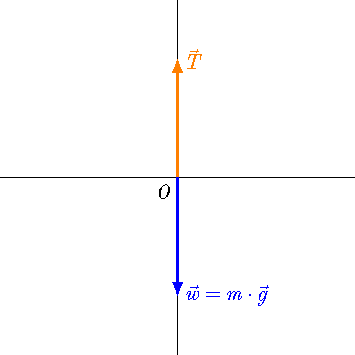
\includegraphics[width= 0.4 \linewidth]{4_APENDICE/1/tikz.pdf}
		\caption{DCL de la situación el portapesas.}
		\label{fig:dcl}
	\end{figure}\\
 	Para el primer sistema, la masa total fue de $ 155 g=0.155 kg $. Por ende, la tensión en la cuerda era de 
 	$$T_1=(0.155 kg)\cdot \left(9.81\frac{m}{s^2}\right)=1.5205 Nw$$
 	Con este valor, y con los datos experimentales obtenidos, se obtuvo lo siguiente
 	\begin{align*}
 		v_a=\lambda\cdot f&=[(134\pm0.05)cm]\cdot[(29\pm 0.05)Hz]=\\
 		&=[(134\cdot29)\pm(134\cdot0.05+ 29\cdot0.05)]\left(\dfrac{cm}{s}\right)=\\
 		&=(3886\pm8.15)\dfrac{cm}{s}
 	\end{align*}
 	Por otro lado, como
 	\begin{align*}
 		\dfrac{T_1}{\mu}&=\dfrac{1.52055 Nw}{(0.00108\pm 0.00001)\dfrac{kg}{m}}=\\\\
 		&=\left[\dfrac{1.52055}{0.00108}\pm\left(1.52055\cdot\dfrac{0.00001}{0.00108^2}\right)\right]\left(\dfrac{\dfrac{kg\cdot m}{s^2}}{\dfrac{kg}{m}}\right)=\\\\
 		&=(1400.173\pm19.65804)\dfrac{m^2}{s^2}
 	\end{align*}
 	
 	Haciendo uso de (\ref{rc}), resulta que
 	\begin{align*}
 		v_b&=\sqrt{\dfrac{T}{\mu}}=\sqrt{(1400.173\pm19.65804)\dfrac{m^2}{s^2}}\\\\
 		&=\left(\sqrt{1400.173}\pm\dfrac{19.65804}{2\cdot\sqrt{1400.173}}\right)\dfrac{m}{s}=\\\\
 		&=(37.41889\pm 0.26267)\dfrac{m}{s}=\\\\
 		&=(3741.889\pm 26.26753)\dfrac{cm}{s}
 	\end{align*}
 
 	Así pues
 	\begin{center}
 		\begin{multicols}{2}
	 		$ v_a=(3886\pm8.15)\dfrac{cm}{s} $\\
	 		$ v_b=(3741.889\pm 26.26753)\dfrac{cm}{s} $
	 	\end{multicols}
 	\end{center}
 	
 	$$\therefore |v_a-v_b|=\left|3886-3741.889\right|\frac{cm}{s}=144.111\frac{cm}{s}$$
 	
 	Similarmente, para el segundo sistema, la masa total fue de $ 205g=0.205kg $, por lo que la tensión de la cuerda resulta de
 	$$T_2=(0.205 kg)\cdot \left(9.81\frac{m}{s^2}\right)=2.01105 Nw$$ 
 	y con los datos experimentales, se tiene que
 	
 	\begin{align*}
 		v_a=\lambda\cdot f&=[(131\pm0.05)cm]\cdot[(33.7\pm 0.05)Hz]=\\
 		&=[(131\cdot33.7)\pm(131\cdot0.05+ 33.7\cdot0.05)]\left(\dfrac{cm}{s}\right)=\\
 		&=(4414.7\pm8.235)\dfrac{cm}{s}
 	\end{align*}
 	Por otro lado
 	\begin{align*}
 		\dfrac{T_2}{\mu}&=\dfrac{2.01105 Nw}{(0.00108\pm 0.00001)\dfrac{kg}{m}}=\\\\
 		&=\left[\dfrac{2.01105}{0.00108}\pm\left(2.01105\cdot\dfrac{0.00001}{0.00108^2}\right)\right]\left(\dfrac{\dfrac{kg\cdot m}{s^2}}{\dfrac{kg}{m}}\right)=\\\\
 		&=(1851.842\pm25.99934)\dfrac{m^2}{s^2}
 	\end{align*}
 	
 	Nuevamente haciendo uso de (\ref{rc}), se obtiene que
 	\begin{align*}
 		v_b&=\sqrt{\dfrac{T}{\mu}}=\sqrt{(1851.842\pm25.99934)\dfrac{m^2}{s^2}}\\\\
 		&=\left(\sqrt{1851.842}\pm\dfrac{25.99934}{2\cdot\sqrt{1851.842}}\right)\dfrac{m}{s}=\\\\
 		&=(43.03303\pm 0.34740)\dfrac{m}{s}=\\\\
 		&=(4303.303\pm 34.74093)\dfrac{cm}{s}
 	\end{align*}
 	
 	Entonces
 	\begin{center}
 		\begin{multicols}{2}
 			$ v_a=(4414.7\pm8.235)\dfrac{cm}{s} $\\
 			$ v_b=(4303.303\pm 34.74093)\dfrac{cm}{s} $
 		\end{multicols}
 	\end{center}
 	
 	$$\therefore |v_a-v_b|=\left|4414.7-4303.303\right|\frac{cm}{s}=111.397\frac{cm}{s}$$
 	
 	\subsection{--- Nueva Estimación para $ \mu $ ---}
	\label{sub:nueva_estim}
 	
 	A partir de la relación 
 	$$T=\left(4\mu f\,^2 L^2\right)\left(\dfrac{1}{n^2}\right)$$
 	se puede decir que
 	$$\mu=\dfrac{Tn^2}{4f\,^2L^2}$$
 	
 	Luego, de la estimación para la recta por mínimos cuadrados (calculada con el software R), se obtuvo 
 	$$ T=[(14.90009\pm 2.29002) Nw]\left(\dfrac{1}{n^2}\right)-(0.06533\pm 0.15625) Nw $$
 	
 	El valor de la pendiente $a=(14.90009\pm 2.29002) Nw$ representa el valor de $ Tn^2 $, puesto que
 	$$a=\dfrac{\Delta y}{\Delta x}=\dfrac{T}{\dfrac{1}{n^2}}=Tn^2$$ 
	y además, de los datos experimentales se tiene que \\[2mm]
	\[
		\begin{array}{lcccl}
			f = (22 \pm 0.05) Hz & \;\implies\; & f\,^2&=&(22\pm0.05)\cdot(22\pm0.05)Hz^2\\
			&&&=&(22^2\pm2\cdot22\cdot0.05)\dfrac{1}{s^2}=(484\pm2.2)\dfrac{1}{s^2} \\[5mm]
			L=(2.67\pm0.0005)m & \;\implies\; & L^2 & = & (2.67\pm0.0005)\cdot(2.67\pm0.0005)m^2 \\[2mm]
			&&& = & (2.67^2\pm2\cdot2.67\cdot0.0005)m^2=(7.1289\pm0.00267)m^2
		\end{array}
		\]
 	
 	Entonces
 	\begin{align*}
 		4f\,^2L^2&=4\left[(484\pm2.2)\dfrac{1}{s^2}\right]\left[(7.1289\pm0.00267)m^2\right]\\
 		&=(1936\pm8.8)(7.1289\pm0.00267)\dfrac{m^2}{s^2}\\
 		&=[1936\cdot7.1289\pm(1936\cdot0.00267+8.8\cdot7.1289)]\dfrac{m^2}{s^2}\\
 		&=(13801.55\pm 67.90344)\dfrac{m^2}{s^2}
 	\end{align*}
 
 	Y así
 	\begin{align*}
 		\mu&=\dfrac{Tn^2}{4f\,^2L^2}=\dfrac{(14.90009\pm 2.29002)}{(13801.55\pm 67.90344)}\dfrac{\dfrac{kg\cdot m}{s^2}}{\dfrac{m^2}{s^2}}\\\\
 		&=\left[\dfrac{14.90009}{13801.55}\pm\left(\dfrac{2.29002}{13801.55}+14.90009\cdot\dfrac{67.90344}{13801.55^2}\right)\right]\dfrac{kg}{m}\\\\
 		&=(0.00107\pm0.0001)\dfrac{kg}{m}
 	\end{align*}
% )))

\end{document}
